This chapter discusses the general architecture of the parallella board, it's memory handling, the development stages, and the tools provided by Adapteva. The aim of this chapter is to have a global overview of the parallella board and the necessary key concepts to start developing on the parallella.

\section{Introduction}

Parallella was launched in 2012 by the Adapteva company. It is the first product based on the \gls{epiphany} architecture, providing a high-performance, energy-efficient and manycore architecture for real-time embeded systems. The Parallella aims to meet 5 constraints \cite{kickstarting} :

\begin{itemize}
  \item Energy efficiency
  \item High raw performance
  \item Scalable to thousands of cores
  \item Emplementable by a team of 5 engineers
\end{itemize}

Facing a huge quest for more computation performance, we are now moving on integration of manycore architecture on a single chip, sometimes called multicore or manycore architecture. A manycore architecture, like the Parallella, consists of a high number of cores. What makes it special is the way those cores can interact together connected as a mesh network, and how they easily provide scalable architecture.

Parallella is a credit card size computer containing 16 \gls{epiphany} cores (\glspl{eCore}). The development of this board was financed in 2102 with a crowd founding website called Kickstarter. In less than 30 days, Adapteva had raised close to 1M USD, making them the first semiconductor company in history to successfully crowd-fund development\cite{kickstarting}. Figure \ref{fig parallella} is a close look at a parallella.

\begin{figure}[h!]
\centering
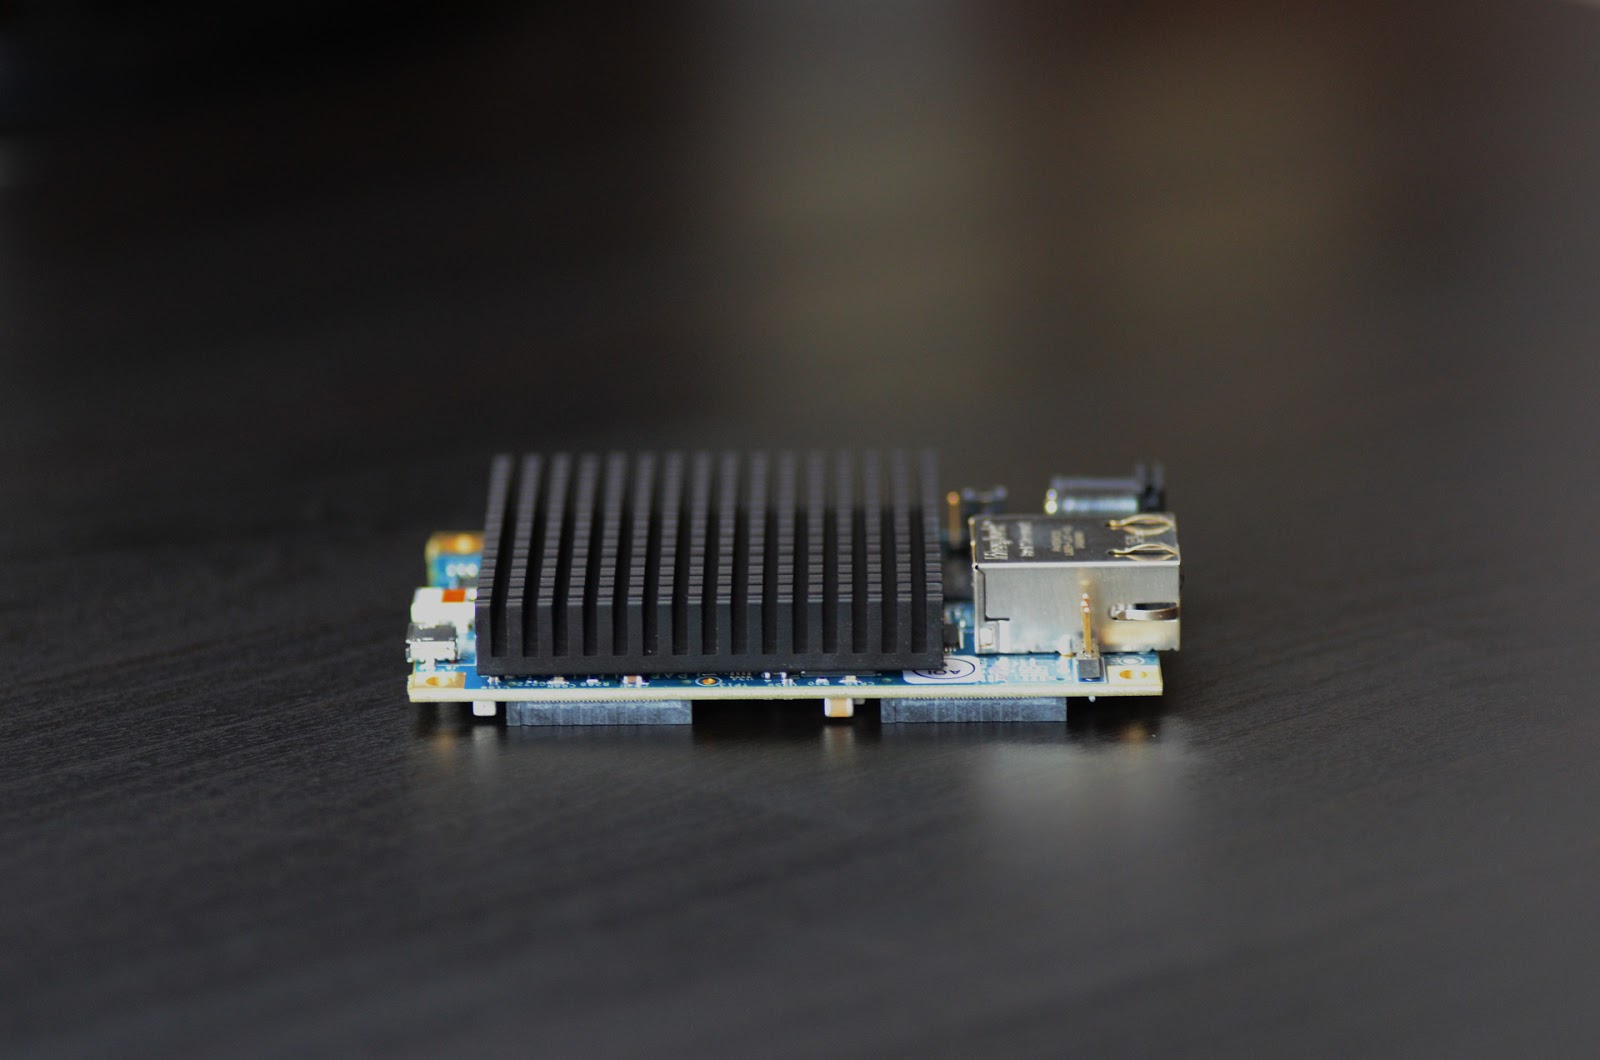
\includegraphics[width=0.5\textwidth]{parallella}
\caption{A close look at the parallela board}
\label{fig parallella}
\end{figure}

In this document, we are going to discover how we can exploit the potential of Parallella by studying it's architecture and developing some test-purposes programs.

\section{Architecture} \label{architecture}
The parallella board includes a 866MHz dual-core ARM-A9 Zynq System-On-Chip and the Adapteva's \gls{epiphany} multicore coprocessor \cite{parallellamanual}. There are 3 different models of the parallella. The "Desktop" and the "Microserver" version with a Xilinx Zynq Dual-core ARM A9 XC7Z010 and an "Embeded" version with a Xilinx Zynq Dual-core ARM A9 XC7Z020. The main differences between them are the host processor versions and the \gls{FPGA} specification. 

The central processor is the Zynq 7000 AP SoC, which is a processor combining a standard ARM dual-core along with an \gls{FPGA}. As shown in figure \ref{fig architecture}, the Zynq chip hosts an \gls{FPGA} which assumes the communication between the Adapteva's \gls{epiphany} multicore side and the host side. The host side is seen as the Zynq board, which hosts the ARM processor, the memory as well as the peripherals.

\begin{figure}[h!]
\centering

\includegraphics[width=0.5\textwidth]{architecture}
\caption{The architecture of a Parallella board}
\label{fig architecture}
\end{figure}

The \gls{epiphany} multicore coprocessor consists of a 2D squared grid composed by 16 \gls{epiphany} cores (\glspl{eCore}). Each \gls{eCore} is linked with its neighbors to compose a networked set of \glspl{eCore}. Figure \ref{fig coprocessor} shows how each \gls{eCore} is assembled as a mesh network. Each node is an \gls{eCore} that acts as a network router as well. Write transactions between \glspl{eCore} can work at an operating frequency of 1GHz and with a latency of 1.5 clock cycles per routing hop\cite{epiphanyArch}. A transaction traversing from the left edge to right edge of a 16 \glspl{eCore} grid would thus take 6 clocks.

\begin{figure}[h!]
\centering
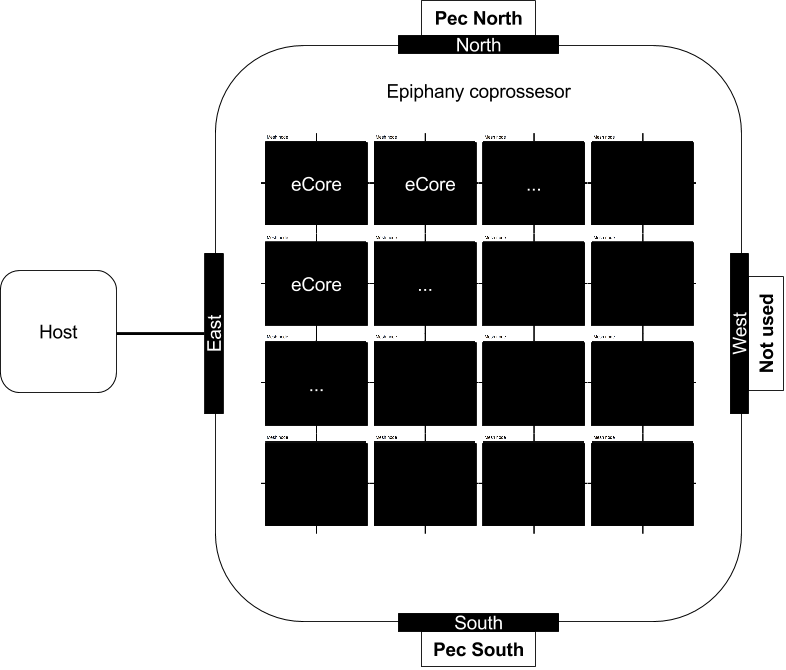
\includegraphics[width=0.5\textwidth]{coprocessor}
\caption{16 cores assembled as a grid and composing the coprocessor of the parallella board}
\label{fig coprocessor}
\end{figure}

Figure \ref{fig eCore} gives a closer look and shows what is contained in a single \gls{eCore}. It is interesting to see that each \gls{eCore} has it's own registers, \gls{DMA}, local memory and everything to compute floating point operations. The local memory is not directly situated on the \gls{eCore}, but mapped from the host memory\cite{parallellamanual}. Data can be routed among \glspl{eCore}, meaning that each \gls{eCore} has its own network interface that are capable of routing data.

\begin{figure}[h!]
\centering
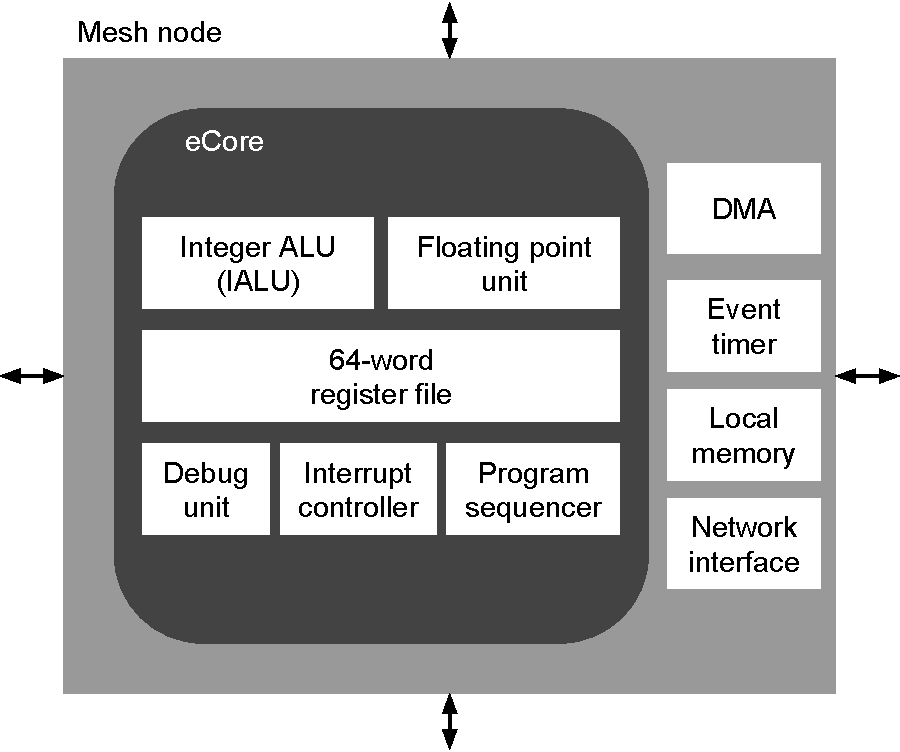
\includegraphics[width=0.6\textwidth]{eCore2.pdf}
\caption{The architecture of a single \gls{eCore}}
\label{fig eCore}
\end{figure}

\section{Memory} \label{memory}
The Zinq chip offers 1GB of DDR3 Memory to the \gls{epiphany}, mapping it from \code{0x8000'0000} to \code{0xBFFF'FFFF}, each addresses giving a 32-bit memory space. The equation \ref{eq:1gb} shows us how to obtain the 1GB space.
\begin{equation}
	2^{7\cdot4+2} \cdot 32 = 1,073,741,824
\label{eq:1gb}
\end{equation}

The \gls{epiphany} architecture uses 32-bit words to address memory, each of whose are word-aligned. It means that each addresses are divisible by 4, giving 4 bytes by words to address.
Each \gls{eCore} has its own local memory accessible from \code{0x0000} to \code{0x7FFF}. That memory is aliased from the global memory. Each eCore also have a globally addressable ID to ensure communication with all other \glspl{eCore}. The \gls{eCore} ID is composed with 6-bits to address row and 6-bits to address column in the grid. Hence allowing a maximum of 4096 \glspl{eCore} in the grid (see equation \ref{eq:4096}). Those bits are situated at the upper most-significant bits (MSB) of the address space.
\begin{equation}
	2^{6+6} = 4096
\label{eq:4096}
\end{equation}

With space going from \code{0x0000} to \code{0x7FFF}, we see that the address range given for each \gls{eCore} corresponds to 32KB (eq \ref{eq:32KB}), which is splited in 4 bank of 8 Bytes.
\begin{equation}
	2^{12+3} = 32,768
\label{eq:32KB}
\end{equation}

That memory is used to store \glspl{eCore}' local information. However, the memory space for each \gls{eCore} is bigger and table \ref{table:eCore}\cite{epiphanyArch} summarizes the \glspl{eCore}' memory map.

\begin{table}[h]
\centering
\caption{Local memory mapped for each eCore}
\label{table:eCore}
\begin{tabular}{|l|r|l|c|}
  \hline
  Description & Start adress & End adress & Size [Bytes] \\
  \hline
  Interrupt vector bank & 0x00 & 0x3F & 64 \\
  Bank 0 & 0x40 & 0x1FFF & 8K-64 \\
  Bank 1 & 0x2000 & 0x3FFF & 8K \\
  Bank 2 & 0x4000 & 0x5FFF & 8K \\
  Bank 3 & 0x6000 & 0x7FFF & 8K \\
  Reserved & 0x8000 & 0xEFFFF & n/a \\
  Memory Mapped Registers & 0xF0000 & 0xF07FF & 2048 \\
  Reserved & 0xF0800 & 0xFFFFF & n/a \\ 
  \hline
\end{tabular}
\end{table}

An interesting thing shown in table \ref{table:eCore} is that each \gls{eCore}'s registers are accessible via memory mapped registers \cite{parallellamanual}.

\subsection{Real mapping}
A linker description file (\gls{LDF}) specifies where data and portion of code resides. That file is used at the linker stage to create a single executable \cite{linker}. The parallella is shipped with its specific \gls{LDF} and, thanks to open hardware, freely open. All hardware sources are available on Github as a public repository \cite{githubadaptevahard}.

The basic \gls{LDF} that we will use maps the global memory from \code{0x8F00'0000} to \code{0x8FFF'FFFF}. That space range is the shared memory among all \glspl{eCore}. Its size, given by equation (\ref{eq:16MB}) is 16MB.

\begin{equation}
	2^{4\cdot6} = 16,777,216
	\label{eq:16MB}
\end{equation}

Another bank of shared memory if mapped from \code{0x8e00'0000} to\\ \code{0x8eff'ffff}. That bank of memory is not currently used.

\subsection{Data transfer}

When an \gls{eCore} in the top left sends data to an \gls{eCore} in bottom right, data first travel through each intermediate \glspl{eCore} following the same row id. Then, when the column id matches the destination column id, data move along rows. As we saw in the previous section (\ref{memory}), each \gls{eCore} has a global address ID composed with a 6-bit row id and a 6-bit column id. Data are routed using the column and row id. Figure \ref{fig grid} illustrates the path of a data sent from the top left \gls{eCore} to the bottom right \gls{eCore}. The dashed arrows represent what would be the reverse path, which is different than the coming path.

\begin{figure}[h!]
\centering
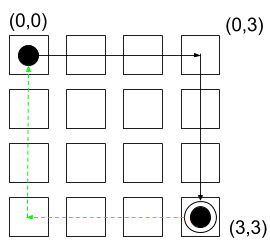
\includegraphics[width=0.4\textwidth]{grid}
\caption{Data path}
\label{fig grid}
\end{figure}

\section{Workflow} \label{workflow}

Programming on the parallella is complex. Because the \gls{epiphany} coprocessor is not directly accessible to code, we must use the host part of the parallella to send \gls{SREC} file to the \gls{epiphany} part. Then, on runtime, the compiled code is sent to the \gls{epiphany} cores. \gls{SREC} files are the only file accepted by the \gls{epiphany} architecture. It a standard assembly file created by Motorola.

We, thus, have two distinct programs : 

\begin{itemize}
  \item the host one, which acts as the main entry point and sends the compiled code to the \gls{epiphany}
  \item the \gls{epiphany} program, which runs on each \gls{eCore} and is sent by the main program
\end{itemize}

Figure \ref{fig workflow} illustrates the principle, where the host part first fetches the compiled \gls{epiphany} code and then deploys it to the \glspl{eCore}.

\begin{figure}[h!]
\centering

\includegraphics[width=0.7\textwidth]{workflow}
\caption{Development workflow}
\label{fig workflow}
\end{figure}

A major downside of this process is that \glspl{eCore}, once deployed, are totally isolated from the host part. Which means that it is impossible to print things from the \glspl{eCore}, thus making debug a bit harder. Communicating between the host and the \gls{epiphany} will only be possible with the aid of shared buffers memory or using local \glspl{eCore}' memory.

\section{Workgroup} \label{workgroup}

It is possible to treat blocs of \glspl{eCore} instead of all at the same time. When deploying source code to the \glspl{eCore}, one can create a workgroup of \glspl{eCore} and only target that workgroup. A workgroup consists of an \glspl{eCore}' rectangle out of the mesh network.

Workgroup has the advantage that a dedicated link is used to move data among \glspl{eCore} of the same workgroup\cite{epiphanyArch}, thus giving faster data transfers. We also use workgroups to manage memory and data transfers. Those points will be discovered in the rest of this document.

Using the provided \gls{SDK}, workgroups are created using \code{e\_open}. This method sets a variable of type \code{e\_epiphany\_t}, which represents a workgroup. This variable will be used to send data to the \glspl{eCore}' workgroup and performing some manipulations on those. We also use workgroup to load \gls{epiphany} specific program (see section \ref{workflow}).

\section{\glspl{SDK}} \label{SDK}

Adapteva provides two \glspl{SDK}, giving out-of-the-box ability to run any application written in ANSI-C. SDK's are :
\begin{itemize}
  \item The Epiphany Hardware Abstract Library (HAL)
  \item The Epiphany Runtime Library (e-lib)
\end{itemize}

The \gls{epiphany} Hardware Abstraction Library (HAL) is meant to be used on the host. It provides methods to initialize the \gls{epiphany} system, create workgroups, start \glspl{eCore} and allocate global memory. That library is the software link between the host part and the \gls{epiphany} part.

The \gls{epiphany} Runtime Library (e-lib) runs on the \glspl{eCore}. It provides many methods to exploit the \gls{epiphany}-specific world like data transactions, interruptions handling, registers accesses, timer manipulation, \gls{DMA} transfers, mutex and barriers functions and workgroup manipulations \cite{epiphanySDK}.

Those \glspl{SDK} must be included in the compilation stage (see next chapter) and are freely available on Github\cite{githubadapteva}. Once done, they can be included with \code{\#include <e-lib.h>} and \code{\#include <e-hal.h>}.

Documentation for those \glspl{SDK} is provided by Adateva and easy to follow. The use of those \glspl{SDK} makes development for the \gls{epiphany} easier, it is a great part of the tools provided for the \gls{epiphany}.

\section{Compiling}

The \gls{epiphany} uses standard c programming environment based on the GNU toolchain\cite{kickstarting}. So, happily, we will use standard tools like the \code{gcc} compiler.

Compiling a program to run on the \gls{epiphany} has several steps. We will first compile the host program with \code{gcc} tool, then compile the \gls{epiphany} specific program, then finally convert the \gls{epiphany} specific compiled code to \gls{SREC} file.

In several examples, Adapteva provides build scripts examples to compile applications. We will comment the main phases.

Compiling host program :

\begin{lstlisting}[language=bash]
${CROSS_PREFIX}gcc main.c -o main.elf  ${EINCS} ${ELIBS} -le-hal -le-loader -lpthread}
\end{lstlisting}

\code{-le-hal} loads the HAL SDK (see section \ref{SDK}). \code{-le-loader} loads the loader utility, responsible of loading programms onto the hardware platform\cite{epiphanySDK}. In our case, that enables us to load our \gls{SREC} file onto \glspl{eCore}. \code{-lpthread} gives access to the linker of the \code{pthread} library.

Compiling \gls{epiphany} program:

\begin{lstlisting}[language=bash]
e-gcc -T ${ELDF} -O${OPT} emain.c -o emain.elf -le-lib
\end{lstlisting}

\code{e-gcc} is based on \code{gcc} and part of the \gls{epiphany} toolchain, it's job is to create a program that is suitable for the \gls{epiphany} architecture. \code{-T} provides a custom linker description file (\gls{LDF}). \code{-O} sets the optimization level, tt can speeds up compilation stage but slow down the runtime.

Convert \gls{epiphany} binary to \gls{SREC} :

\begin{lstlisting}[language=bash]
e-objcopy --srec-forceS3 --output-target srec emain.elf emain.srec
\end{lstlisting}

\code{e-objcopy} is a provided utility to convert binary file to \gls{SREC} file. Provided options sets correct format for the \gls{SREC} file.

The compilation stage is specific and would be a pain without any examples. But fortunately, the parallella is shipped with many examples that help to understand and utilities provided gives a great toolchain for the \gls{epiphany}. The distributions available for the parallella includes by default the \gls{epiphany} toolchain.

\section{Conclusion}

Having an overview of the parallella functionalities took what we planned, about one third of the time allocated for this project. It wasn't always easy to find specific information with the documentation provided by Adapteva. For example, to know the memory mapping, looking at the documentation wasn't enough. We had to browse the hardware sources to find out what we were looking at. Documentation for the \gls{epiphany} architecture\cite{epiphanyArch} is in general quite complete and done well. But the parallella documentation sometimes leaves a feeling of being hastily drawn. Finding books or articles speaking about the parallella didn't give much results, there is only few ones and it is understandable for a rising system like the parallella. For somebody not familiar with the parallella ecosystem, it may take time to find its feet.